% *********************************************************************
% © 2016–2024 Jeremy Sylvestre
%
% Permission is granted to copy, distribute and/or modify this document
% under the terms of the GNU Free Documentation License, Version 1.3 or
% any later version published by the Free Software Foundation; with no
% Invariant Sections, no Front-Cover Texts, and no Back-Cover Texts. A
% copy of the license is included in the appendix entitled “GNU Free
% Documentation License” that appears in the output document of this
% PreTeXt source code. All trademarks™ are the registered® marks of
% their respective owners.
%
% *********************************************************************
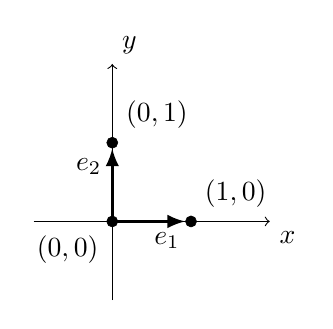
\begin{tikzpicture}[
	point/.style={circle,draw,very thin,fill,inner sep=0pt,minimum size=4pt},
	vector/.style={-latex},
]
	\draw[->] (-1,0) to (2,0) node[below right] {$x$};
	\draw[->] (0,-1) -- (0,2) node[above right] {$y$};

	\node[point] at (0,0) (o) [label=below left:{$(0,0)$}] {};
	\node[point] at (1,0) (e1) [label=above right:{$(1,0)$}] {};
	\node[point] at (0,1) (e2) [label=above right:{$(0,1)$}] {};
	\draw[vector,very thick] (0,0) to node[below, near end] {$\uvec{e}_1$} (e1);
	\draw[vector,very thick] (0,0) to node[left, near end] {$\uvec{e}_2$} (e2);
\end{tikzpicture}
